\chapter{Resultados}

\section{Placas de Circuito Impresso}

As placas de circuito impresso foram produzidas em uma empresa externa \cite{euroC}, utilizando os arquivos gerados no programa EAGLE 7.1 \cite{EagleWiki}. 

A placa para o encaixe do sensor pode ser obsevada na figura \ref{fig:pcbSensor}. A importância dessa placa é a de alinhamento do sensor com a região de interesse no centro da estrutura em conjunto com o suporte do sensor. Emprega um conector que possui boa fixação para diminuir eventuais problemas de conexão. 

A estratégia utilizada no cabo produzido dessa placa foi a de transmitir paralelamente a cada fio de sinal, um fio de referência, trançando levemente os dois cabos para uma diminuição de ruído irradiado. Assim, esse par de fios reduz o efeito produzido pelas correntes de modo comum, onde o campo gerado pelo cabo do sinal é cancelado pelo campo gerado pelo cabo de referência que o acompanha.

\begin{figure}[H]
    \centering
     \caption{Resultado da PCI do sensor.}
     \subfloat[Visão superior.]{%
       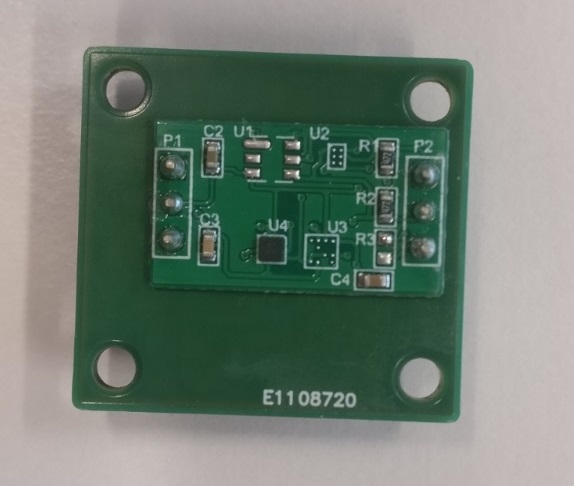
\includegraphics[width=0.51\textwidth]{./img/PCBs/placaSensor.jpg}
     }
     \subfloat[Visão inferior.]{%
       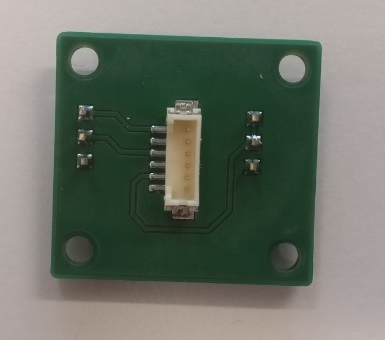
\includegraphics[width=0.49\textwidth]{./img/PCBs/placaSensor1.jpg}
     }
    % \hfill
     \caption*{Fonte: Autor.}\label{fig:pcbSensor}
\end{figure}

A PCI principal do sistema, na qual estão conectados o computador, a fonte, o sensor e as bobinas, é mostrada na figura \ref{fig:pbcMain}. Nessa, a preocupação maior era com a solda dos componentes SMD, pois esse procedimento seria feito de forma manual. Nesse caso, um \textit{stencil} foi utilizado juntamente com um forno elétrico doméstico, facilitando o processo de inserção e soldagem da placa.

Os componentes estão distribuídos espaçadamente na placa para melhor manuseio. A distribuição foi pensada para facilitar as conexões necessárias e uma possível manutenção. Na figura \ref{fig:hardwareSistema} é possível observar o sistema montado com sensor e microcontrolador conectados na placa principal.

\begin{figure}[H]
    \centering
     \caption{Resultado da PCI do sistema}
     \subfloat[Visão superior]{%
       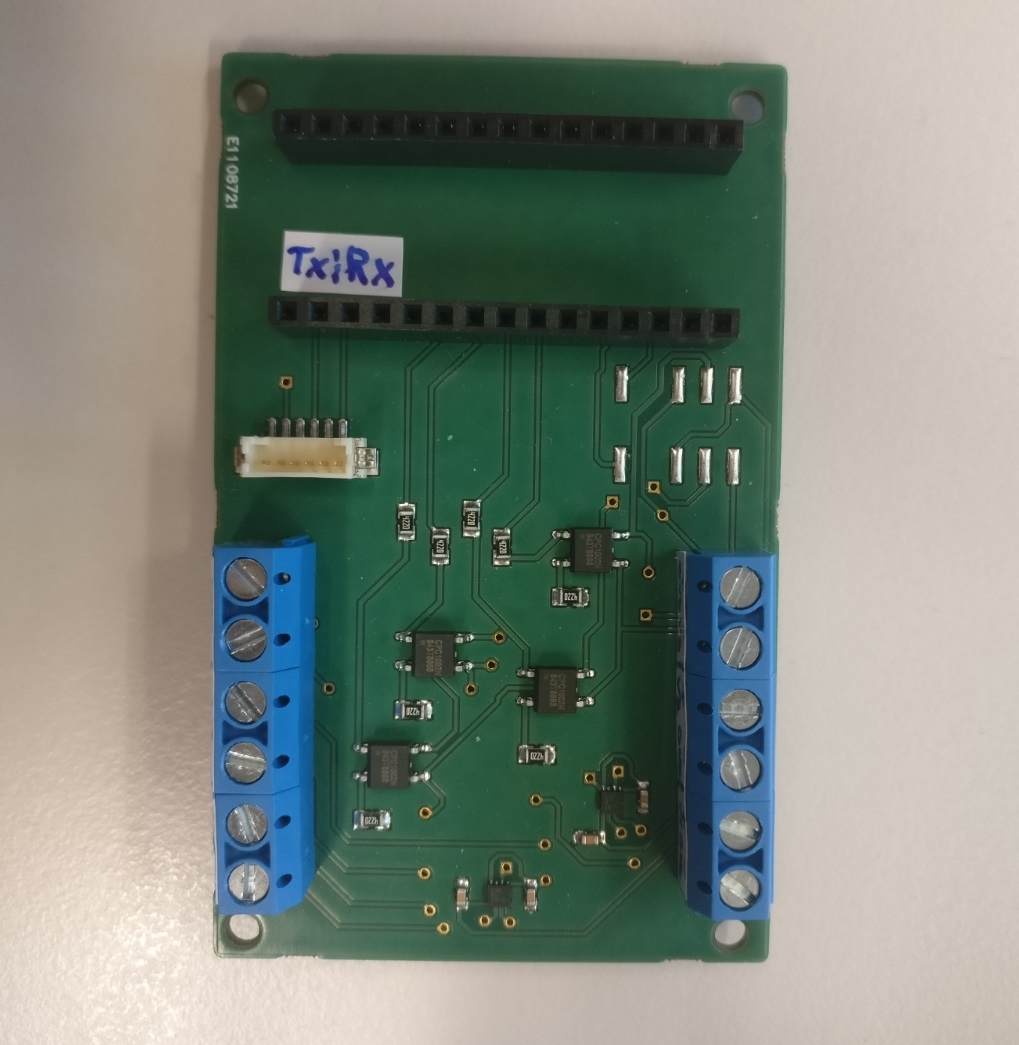
\includegraphics[width=0.51\textwidth]{./img/PCBs/placaMain1.jpg}
     }
     \subfloat[Visão inferior]{%
       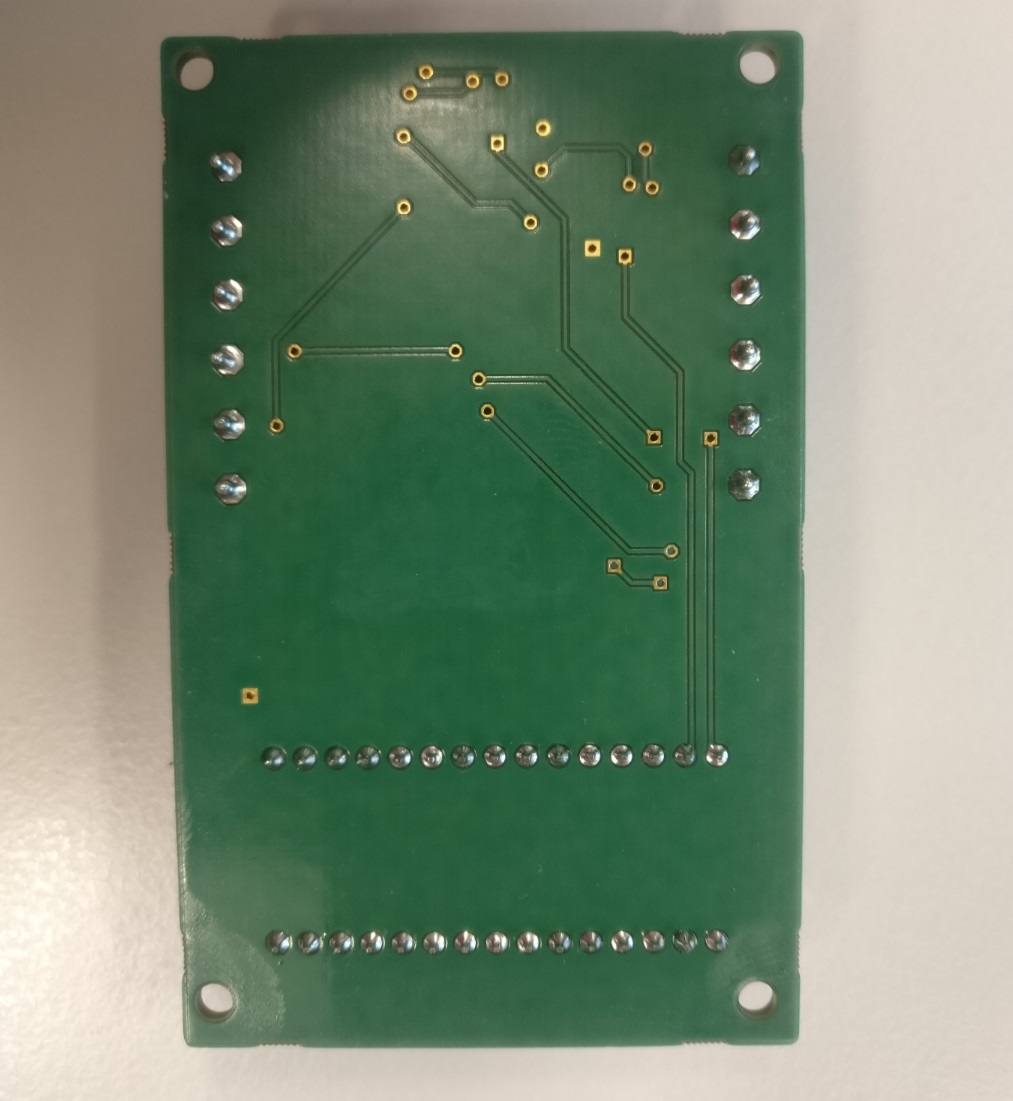
\includegraphics[width=0.48\textwidth]{./img/PCBs/placaMain.jpg}
     }
    % \hfill
     \caption*{Fonte: Autor.}\label{fig:pbcMain}
\end{figure}

\begin{figure}[H]
    \centering
     \caption{Hardware montado.}
     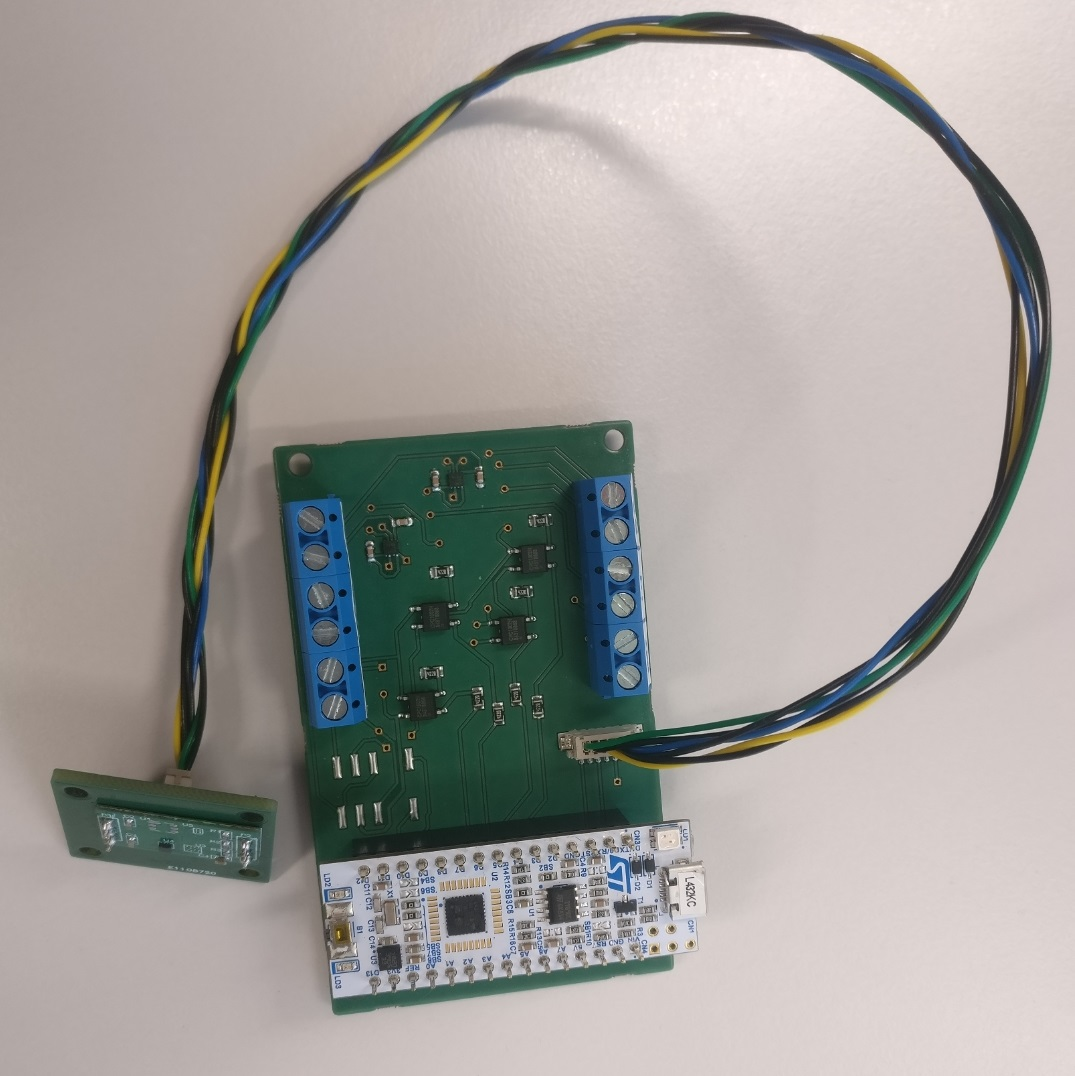
\includegraphics[width=0.55\textwidth]{./img/PCBs/placaMontada.jpg}
     \caption*{Fonte: Autor.}\label{fig:hardwareSistema}
\end{figure}

\section{Impressões 3D}

Para que os resultados obtidos nas simulações fossem alcançados, a impressão das peças tridimensionais deveria ter a maior precisão possível. As impressões realizadas para todas as peças exceto o tripé contam com uma precisão de 0,05 $\mu m$ o que faz desprezível qualquer problema mecânico relacionado a precisão da impressão.

Os resultados das impressões do suporte do sensor e transdutor pode ser observado na figura \label{fig:supsenim} e dos rebites na figura \label{fig:rebim}. Os rebites tem diferença de 50 μm entre seus diâmetros, possibilitando diferentes pressões de fixação do suporte do sensor e transdutor.

\begin{figure}[H]
    \centering
     \caption{Suporte do sensor.}
     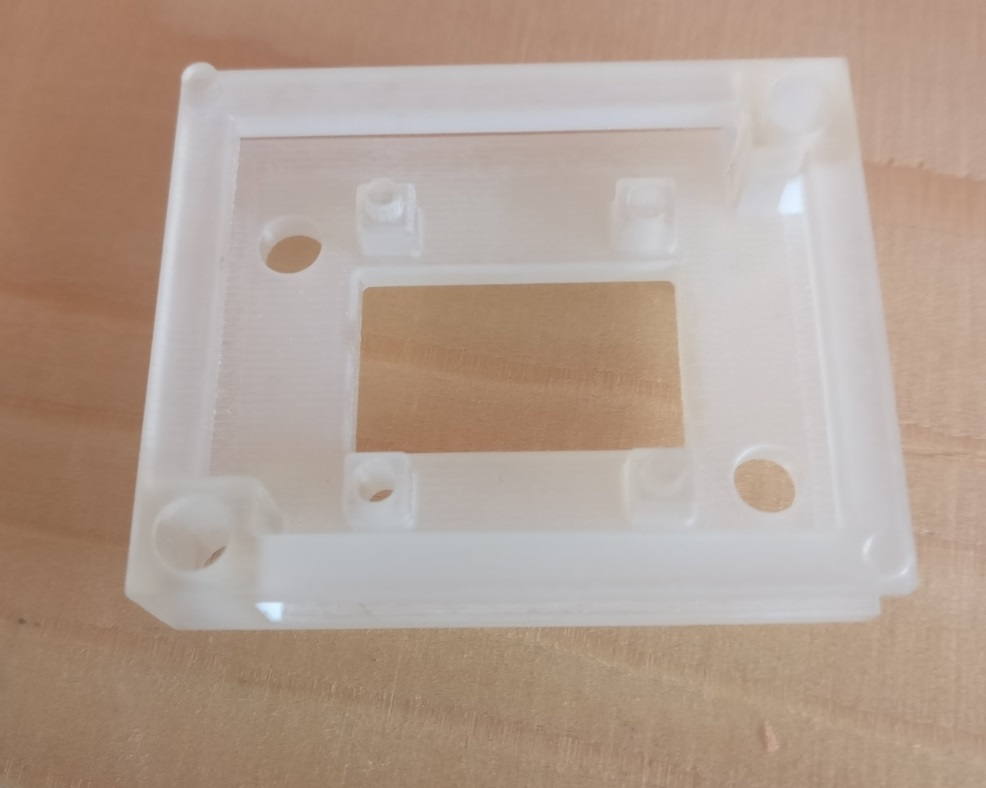
\includegraphics[width=0.55\textwidth]{./img/impressoes3D/suporte_sensor.jpg}
     \caption*{Fonte: Autor.}\label{fig:supsenim}
\end{figure}

\begin{figure}[H]
    \centering
     \caption{Resultado da impressão dos rebites.}
     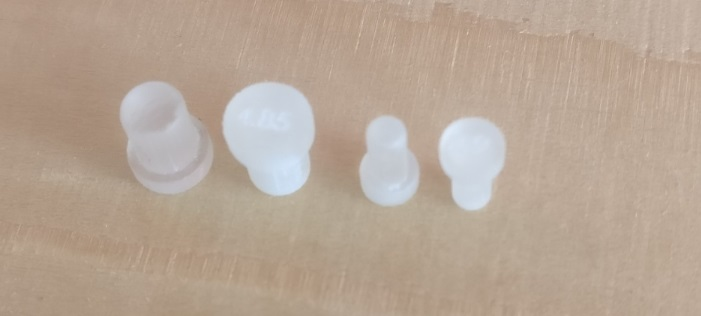
\includegraphics[width=0.55\textwidth]{./img/impressoes3D/rebites.jpg}
     \caption*{Fonte: Autor.}\label{fig:rebim}
\end{figure}

Na impressão do tripé para o suporte das bobinas a precisão da impressora não era relevante para o resultado. O resultado da impressão do tripé pode ser observado na figura \ref{fig:tripim}, o centro do tripé foi projetado para que se encaixe perfeitamente ao suporte das bobinas, com o desenho formado pelos "pés" do suporte. A estrutura impressa do suporte das bobinas pode ser observada na figura \ref{fig:bob}.

\begin{figure}[H]
    \centering
     \caption{Impressão do tripé.}
     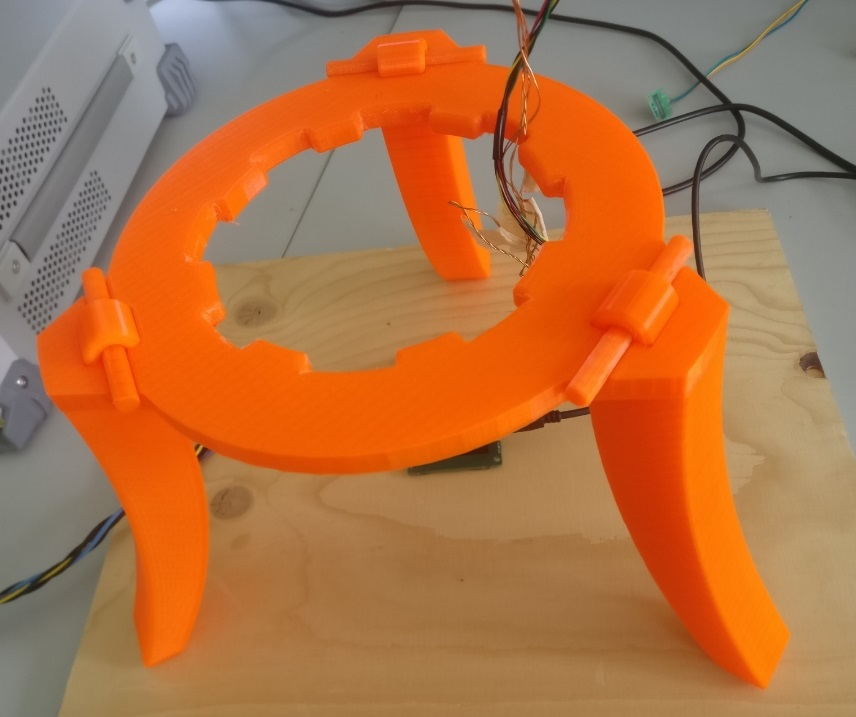
\includegraphics[width=0.5\textwidth]{./img/impressoes3D/tripe.jpg}
     \caption*{Fonte: Autor.}\label{fig:tripim}
\end{figure}

\begin{figure}[H]
    \centering
     \caption{Impressão do suporte para as bobinas 3D}
     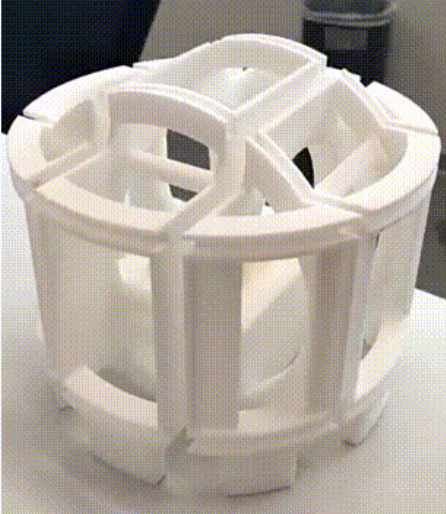
\includegraphics[width=0.5\textwidth]{./img/impressoes3D/bobiba1.jpg}
     \caption*{Fonte: Autor.}\label{fig:bob}
\end{figure}

Na figura \ref{fig:sensup} é possível observar a peça de suporte do sensor encaixada ao suporte das bobinas. A fixação é feita através dos rebites, os quais dão pressão mecânica, o sensor fica posicionado no centro da estrutura, não havendo problemas de movimentação durante as medições.

\begin{figure}[H]
    \centering
     \caption{Encaixe do suporte do sensor}
     \subfloat[]{%
        
     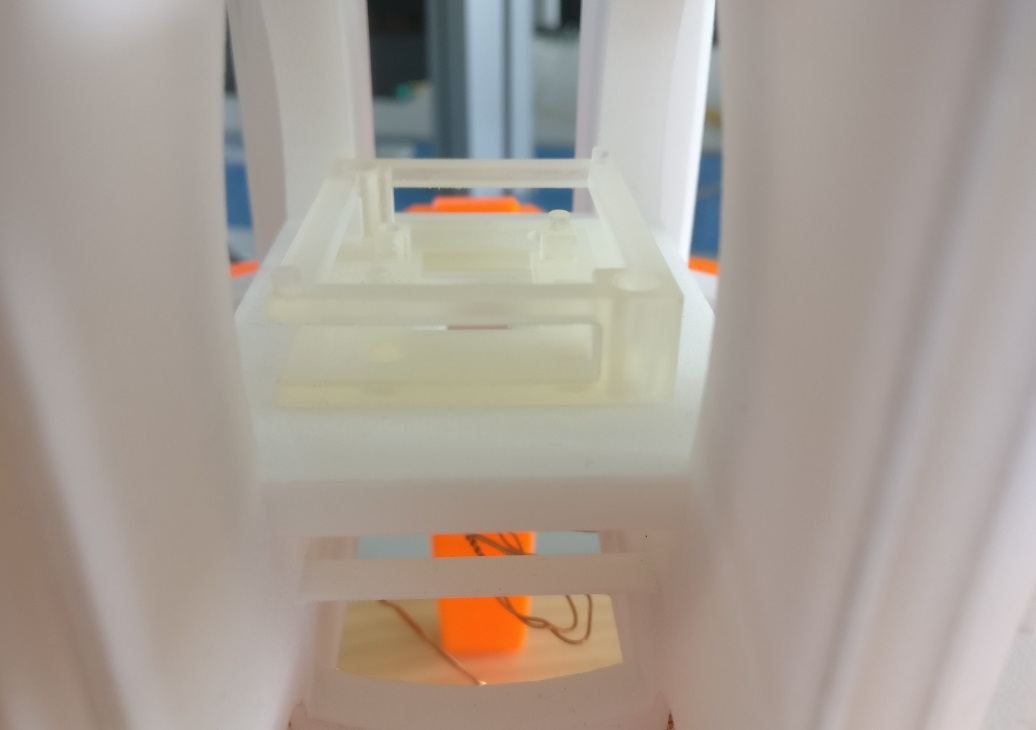
\includegraphics[width=0.45\textwidth]{./img/impressoes3D/encaixe_suporte_sensor.jpg}
     }
     \subfloat[]{%
     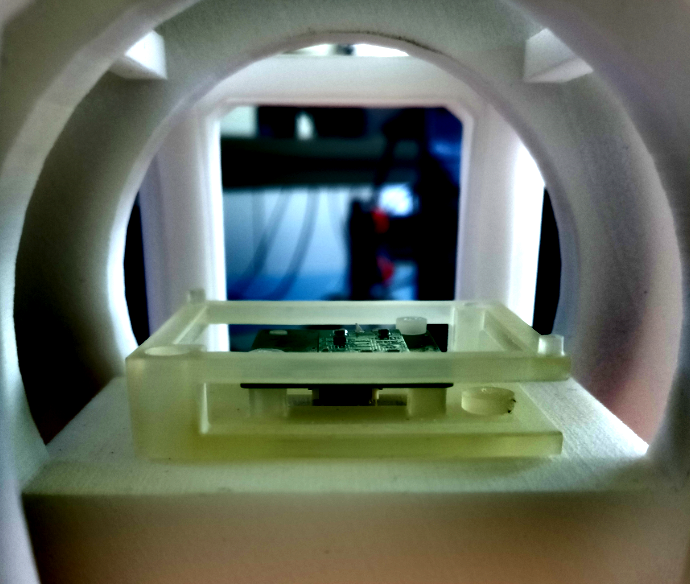
\includegraphics[width=0.38\textwidth]{./img/impressoes3D/encaixe_suporte_sensor 2.png}
     }
     \caption*{Fonte: Autor.}\label{fig:sensup}
\end{figure}


\section{Enrolamento das bobinas}

O enrolamento das bobinas foi realizado de forma simples, utilizando uma morsa de bancada, uma chave de fenda e o próprio rolo de fio. Foi possível gerar uma tensão sobre o fio ao ser esticado, mostrado na figura \ref{fig:morsa} (a). Esse fio ao ser enrolado no suporte das bobinas com essa tensão se encaixa perfeitamente no suporte das bobinas, permitindo que a geometria dos enrolamentos fique quase igual à geometria utilizada no simulador, o que é importante para que a indução real gerada pelas bobinas seja a mais próxima possível da indução verificada nas simulações. Na figura \ref{fig:morsa} (b) é possível observar as bobinas enroladas no suporte.

\begin{figure}[H]
    \centering
     \caption{Enrolamento das bobinas}
     \subfloat[]{%
        
     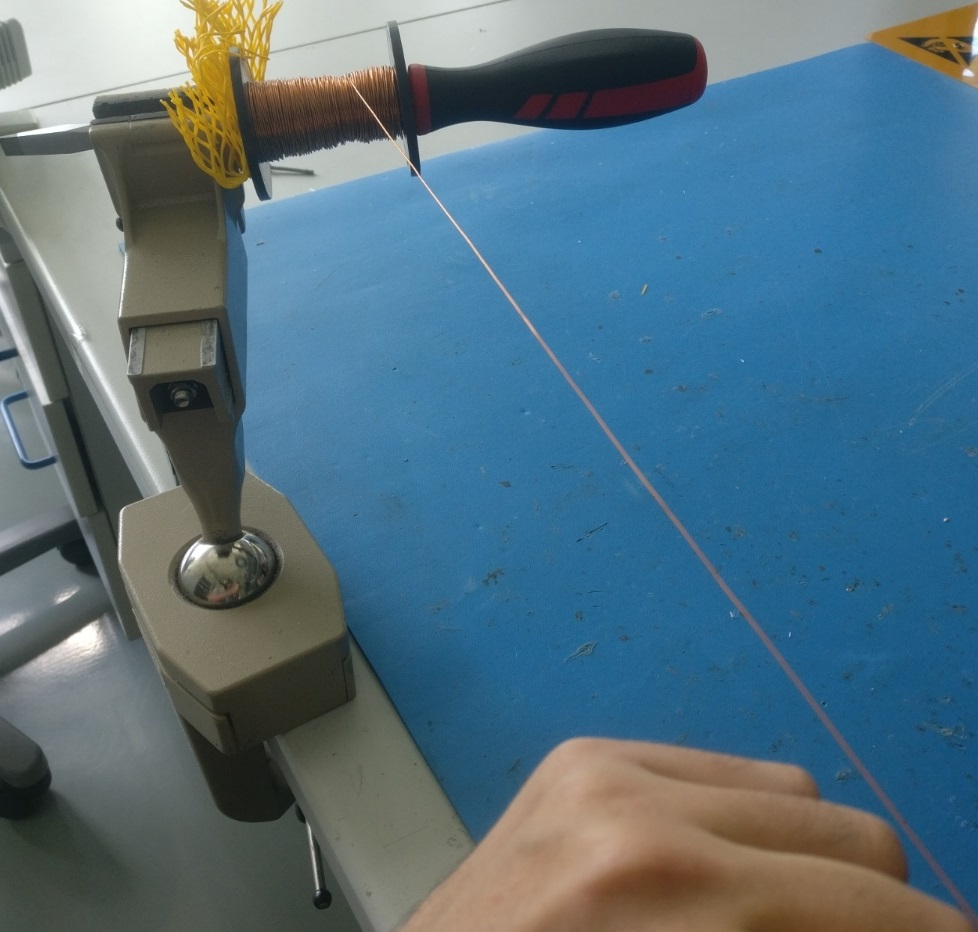
\includegraphics[width=0.45\textwidth]{./img/resultados/morsa.jpg}
     }
     \subfloat[]{%
     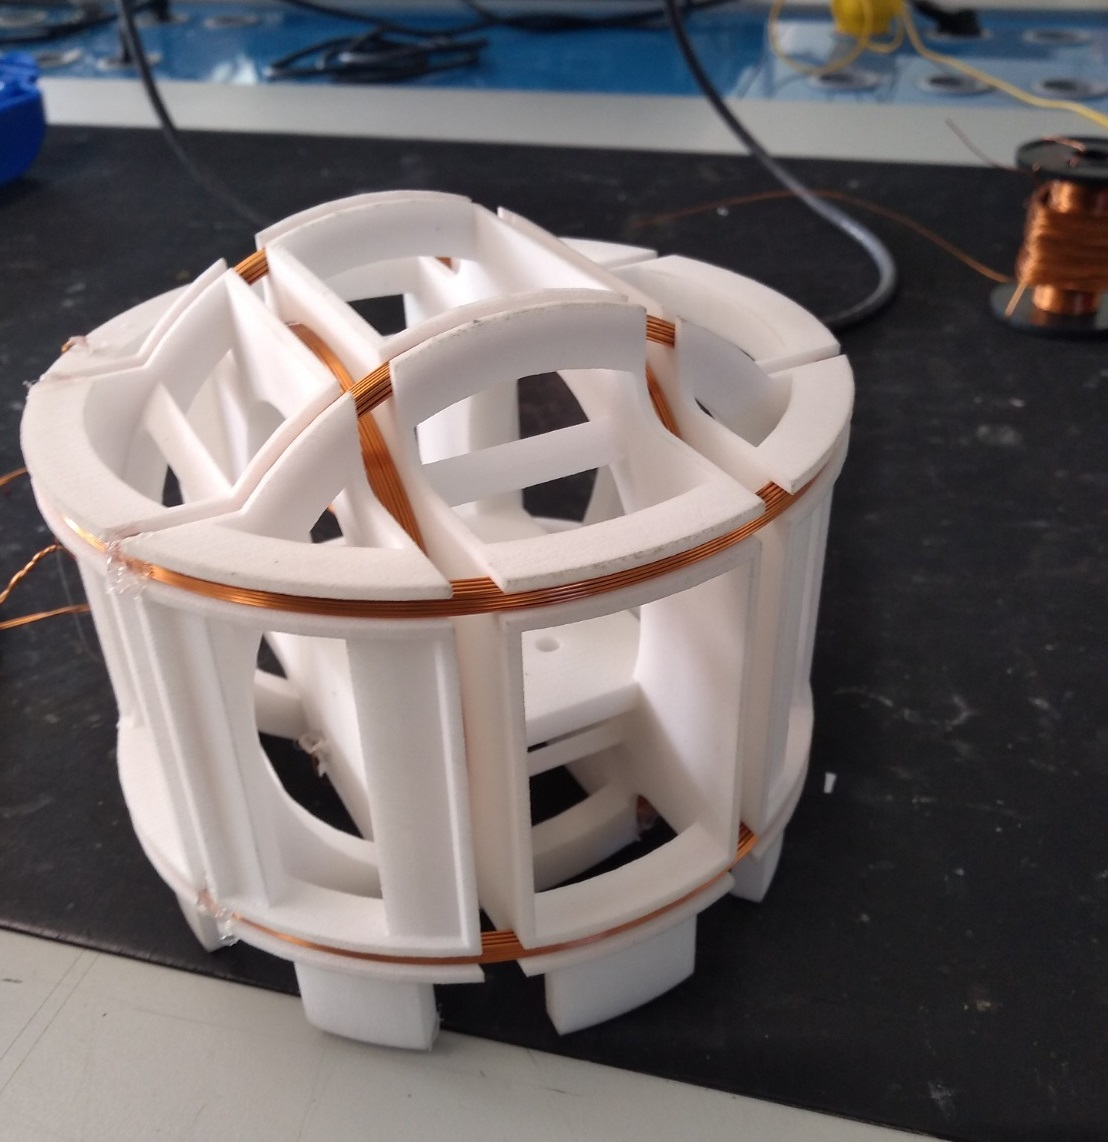
\includegraphics[width=0.415\textwidth]{./img/resultados/bobinas2.jpg}
     }
     \caption*{Fonte: Autor.}\label{fig:morsa}
\end{figure}


\section{Caracterização das bobinas}

Na figura \ref{fig:final} pode ser visualizado o equipamento montado e integrado. Os cabos vindos da fonte de potência são conectados em um lado da placa do sistema, a corrente por eles transmitida passa pelas pontes H, uma para cada canal, saindo pelo outro lado da placa que está conectado diretamente às bobinas. Há uma conexão entre o sensor localizado no meio da estrutura de suporte das bobinas e a placa principal do sistema, feita por um cabo de pares levemente trançados. O microcontrolador da placa do sistema é conectado ao computador através de um cabo USB. A aquisição de dados é recebida por um computador, o qual processa as medidas para que sejam ajustadas para a posição correta.


\begin{figure}[H]
    \centering
     \caption{Equipamento montado e integrado}
     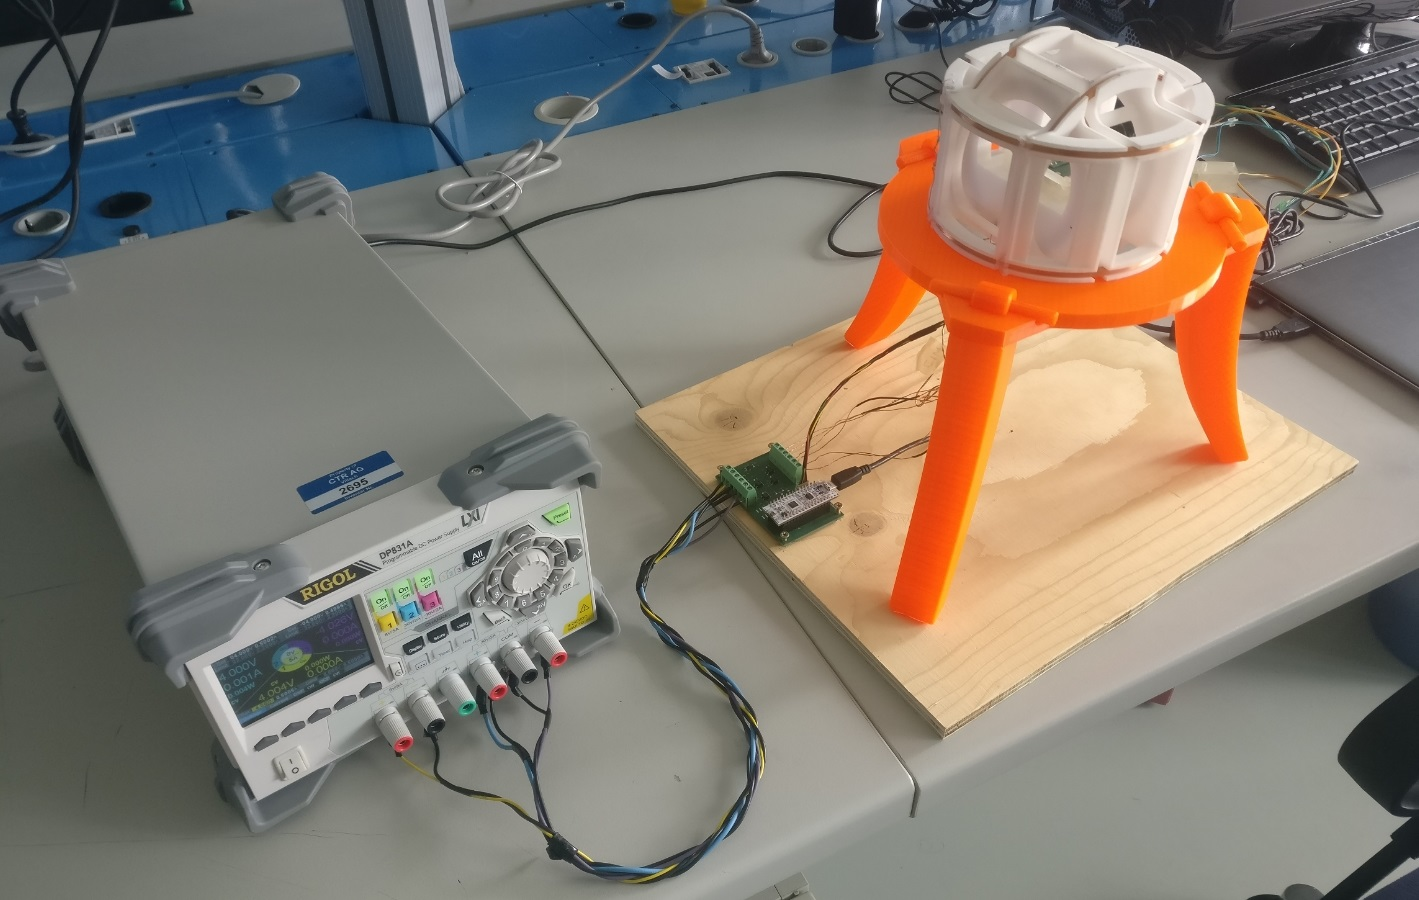
\includegraphics[width=1\textwidth]{./img/resultados/resultSystem.jpg}
     \caption*{Fonte: Autor.}\label{fig:final}
\end{figure}

Na análise das bobinas foi utilizado o sensor magnético MMC3416 posicionado no centro da estrutura de suporte. Então, as medidas em $\muT$ dos eixos x, y e z são enviadas para um computador. As medidas enviadas estão em $\muT$, com medidas em x, y e z respectivamente em cada linha recebida.

\subsection{Bobina interna}

A bobina mais interna, também chamada de bobina principal z, é a bobina que gera o campo mais intenso, com maior número de enrolamentos e maior quantidade de fio. Em comparação com os outros enrolamentos, este tem a maior resistência e indutância. Nas figuras \ref{fig:ResIndIn} e \ref{fig:CurFieldIn} podem ser vistos, para essa bobina, os valores medidos de tensão, corrente, indução magnética, resistência e indutância.

\begin{figure}[H]
    \centering
     \caption{Medidas de resistência e indutância na bobina interna}
     \subfloat[Valor da resistência medida ($\Omega$)]{%
        \includegraphics[width=0.25\textwidth]{./img/bob/innerCoilResistance.jpg}
     }
     \subfloat[Valor da indutância medida (mH)]{%
        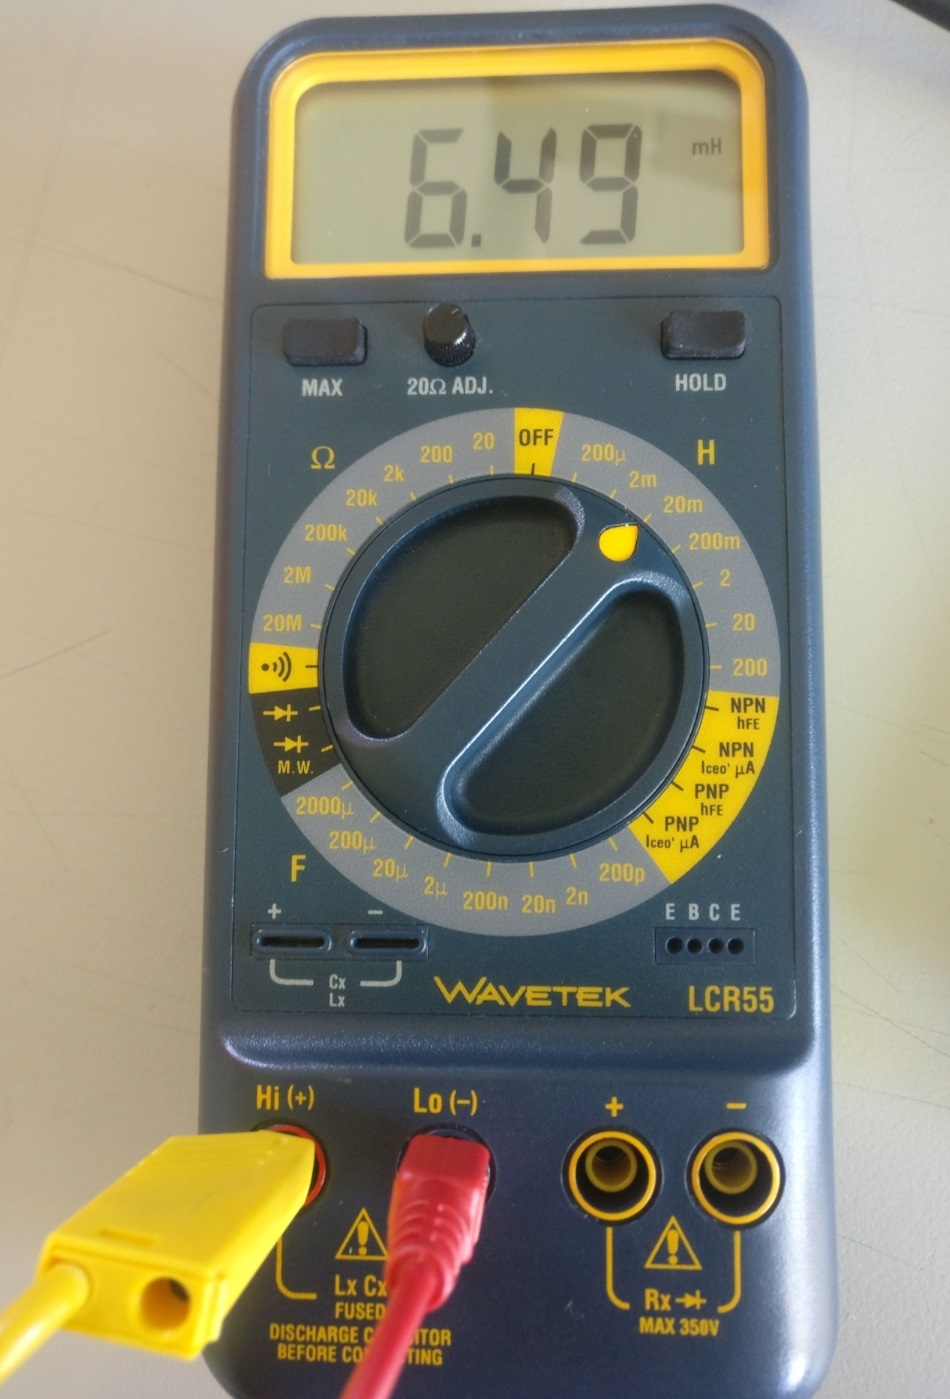
\includegraphics[width=0.24\textwidth]{./img/bob/innerCoilInductance.jpg}
     }
    % \hfill
     \caption*{Fonte: Autor.}\label{fig:ResIndIn}
\end{figure}


\begin{figure}[H]
    \centering
     \caption{Estimação do campo gerado pela bobina interna}
     \subfloat[Tensão e corrente da fonte]{%
        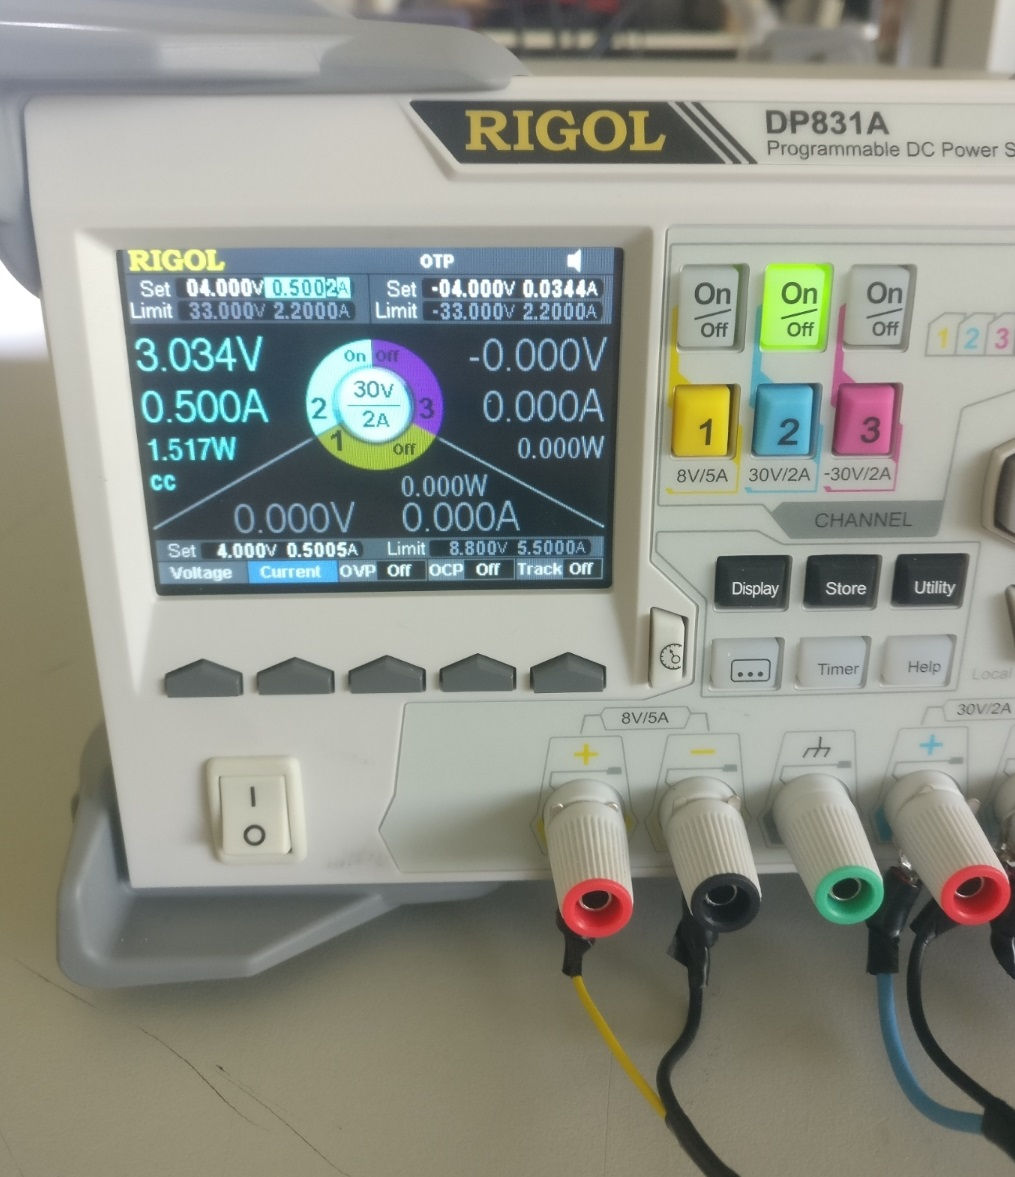
\includegraphics[width=0.35\textwidth]{./img/bob/innerCoilCurrent.jpg}
     }
     \subfloat[Valores de campo recebidos no computador]{%
        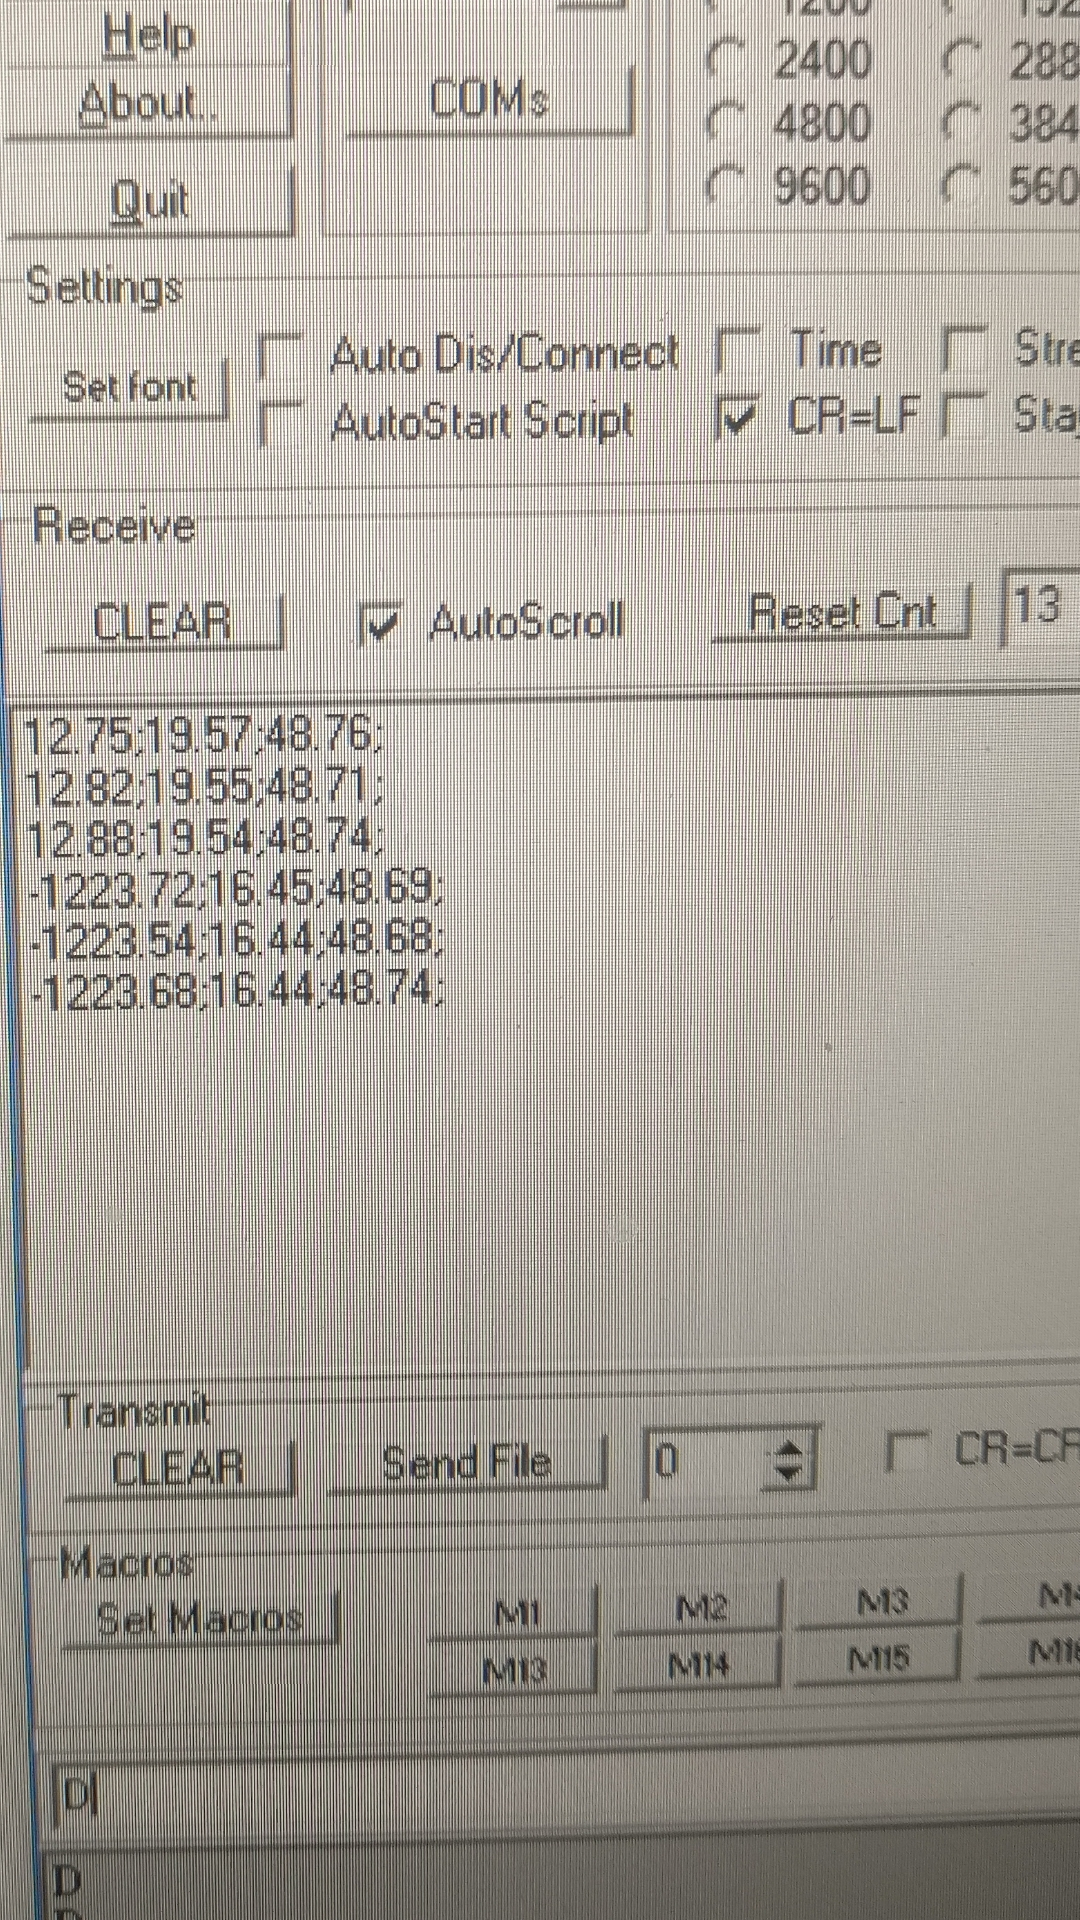
\includegraphics[width=0.23\textwidth]{./img/bob/innerCoilField.jpg}
     }
    % \hfill
     \caption*{Fonte: Autor.}\label{fig:CurFieldIn}
\end{figure}


\subsection{Bobina intermediária e externa}

As medidas de resistência e campo gerado pelas bobinas intermediária e externa podem ser vistas nas figura \ref{fig:ResIndMd}, \ref{fig:CurFieldMd}, \ref{fig:ResIndEx} e \ref{fig:CurFieldEx}.

\begin{figure}[H]
    \centering
     \caption{Medidas de resistência e indutância na bobina intermediária}
     \subfloat[Valor da resistência medida ($\Omega$)]{%
        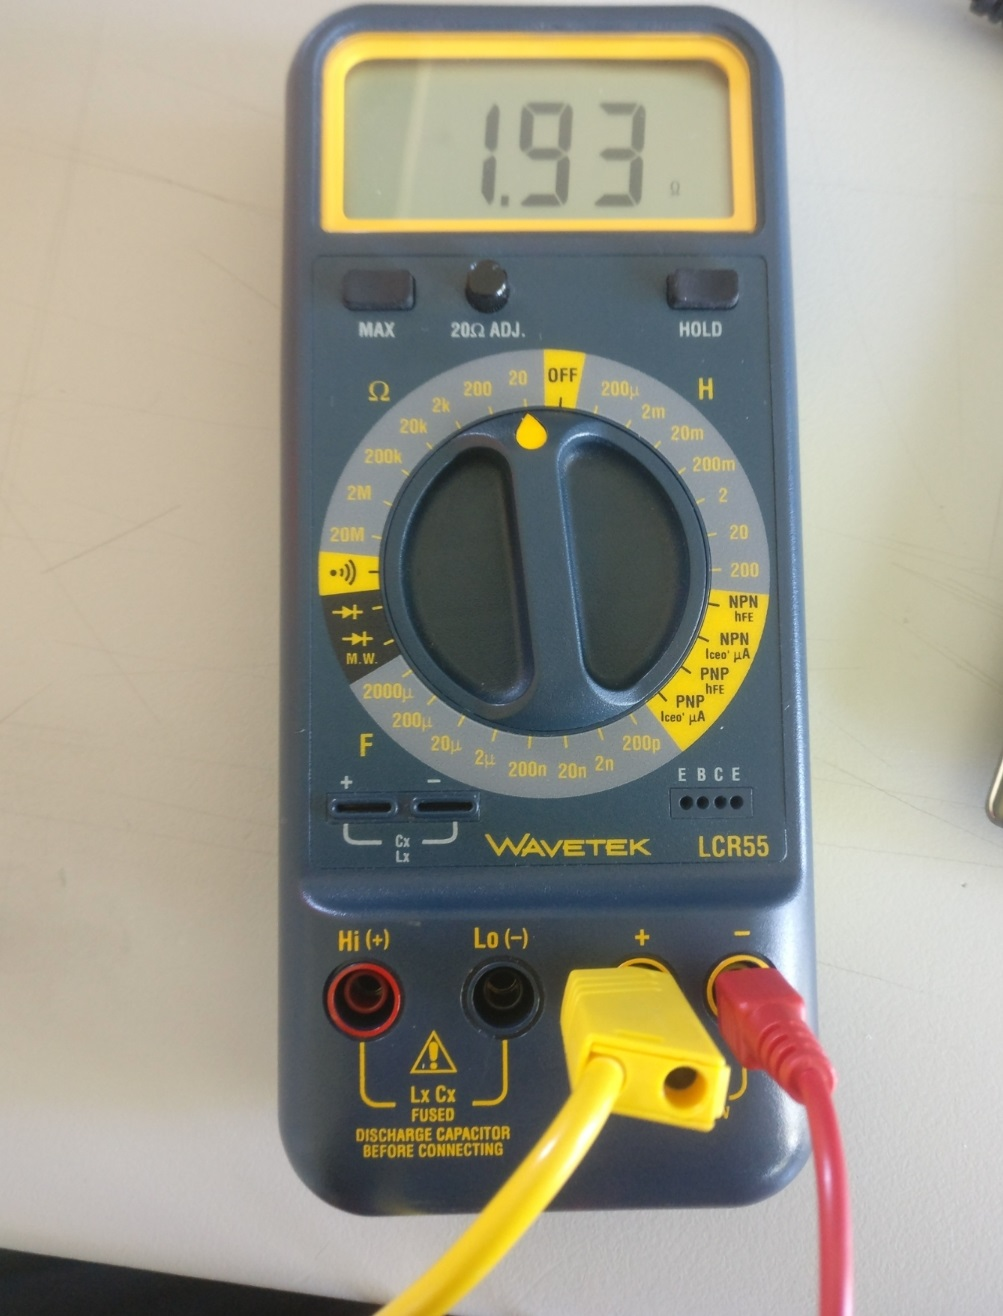
\includegraphics[width=0.26\textwidth]{./img/bob/midCoilResistance.jpg}
     }
     \subfloat[Valor da indutância medida (mH)]{%
        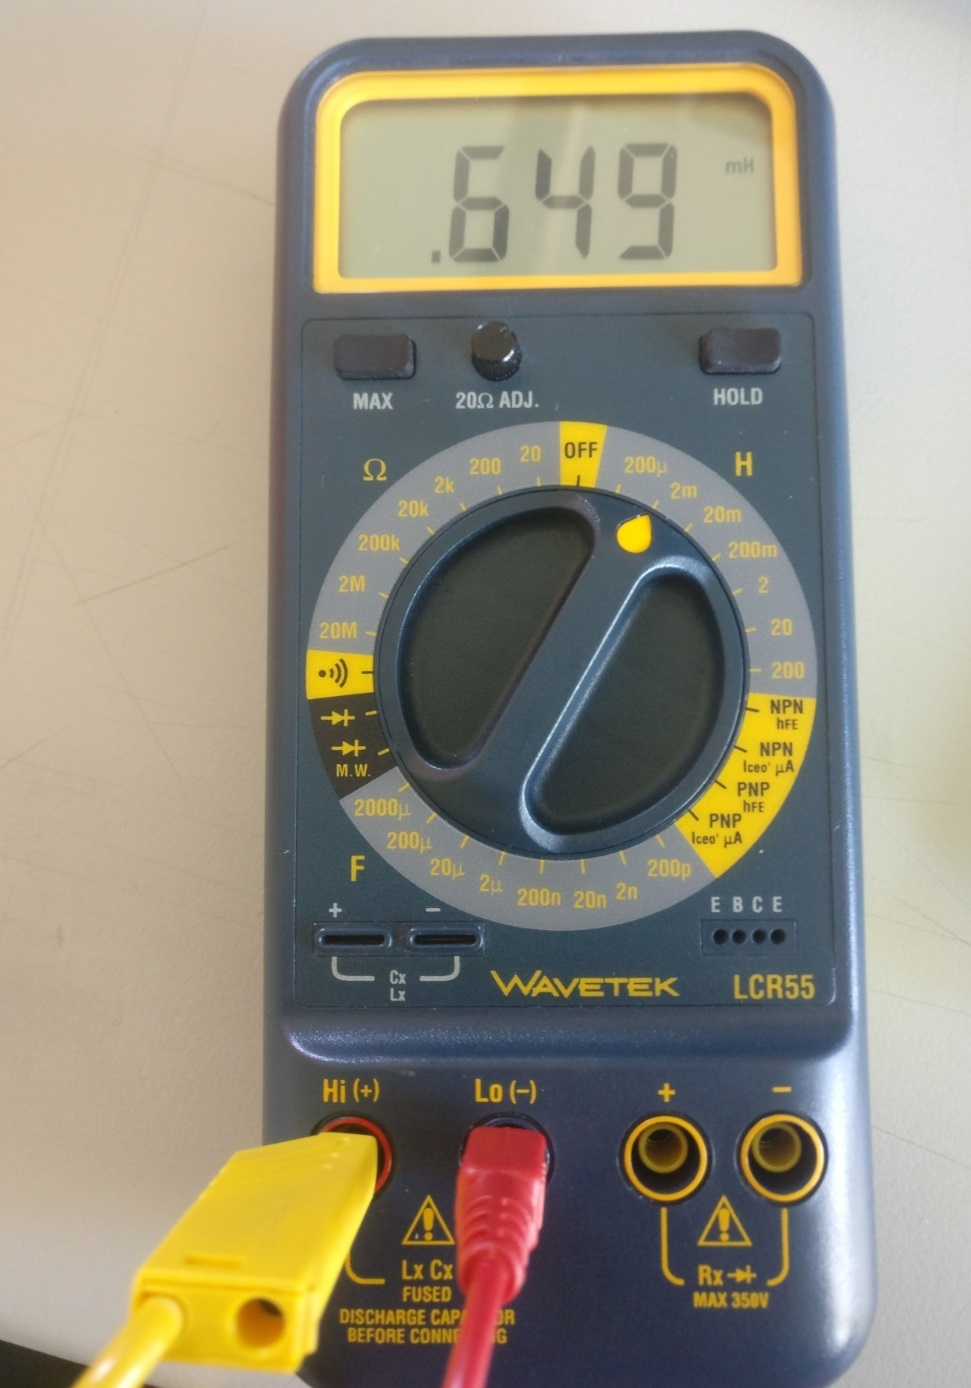
\includegraphics[width=0.24\textwidth]{./img/bob/midCoilInductance.jpg}
     }
    % \hfill
     \caption*{Fonte: Autor.}\label{fig:ResIndMd}
\end{figure}

\begin{figure}[H]
    \centering
     \caption{Estimação do campo gerado pela bobina intermediária}
     \subfloat[Tensão e corrente da fonte]{%
        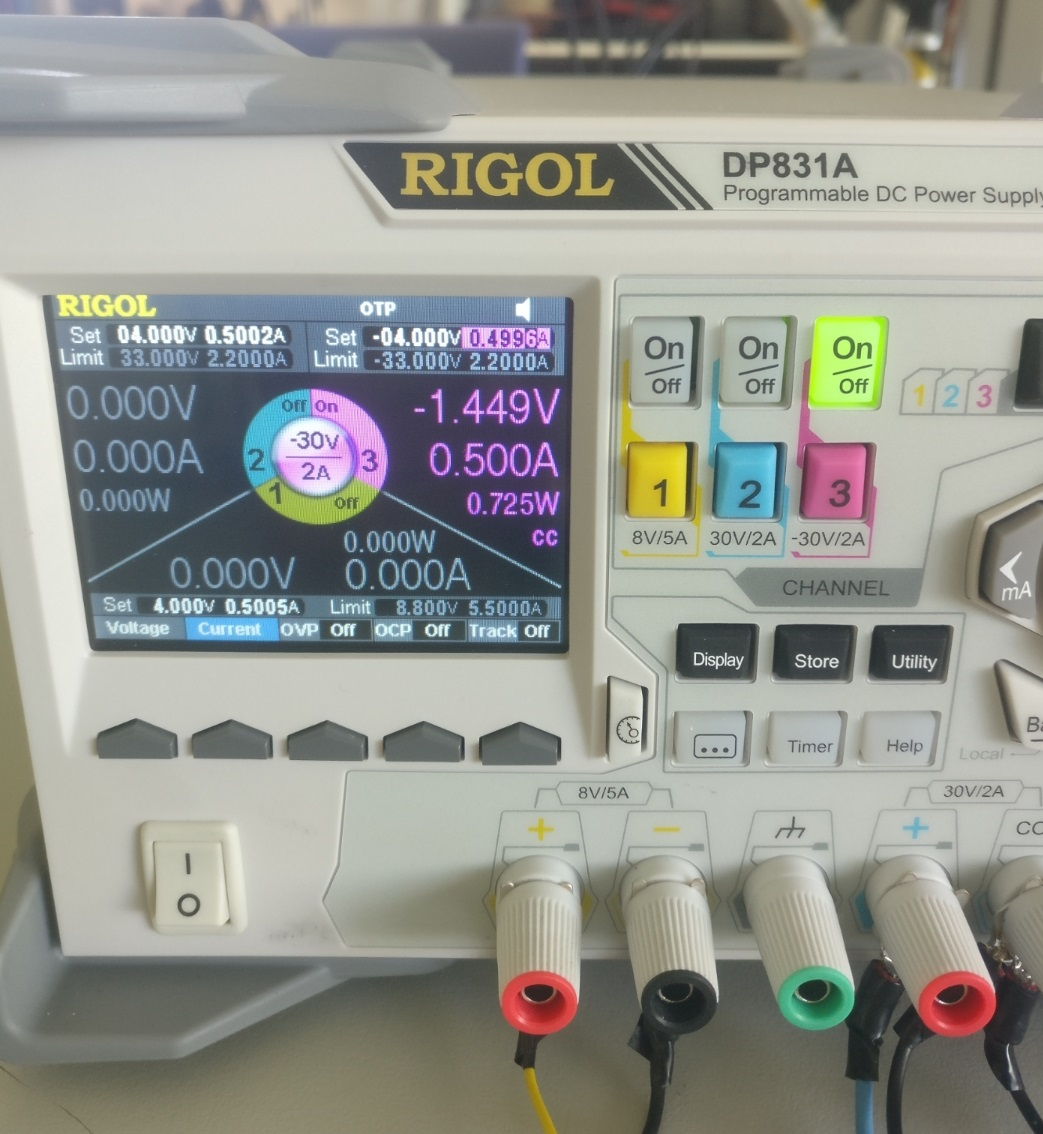
\includegraphics[width=0.35\textwidth]{./img/bob/midCoilCurrent.jpg}
     }
     \subfloat[Valores de campo recebidos no computador]{%
        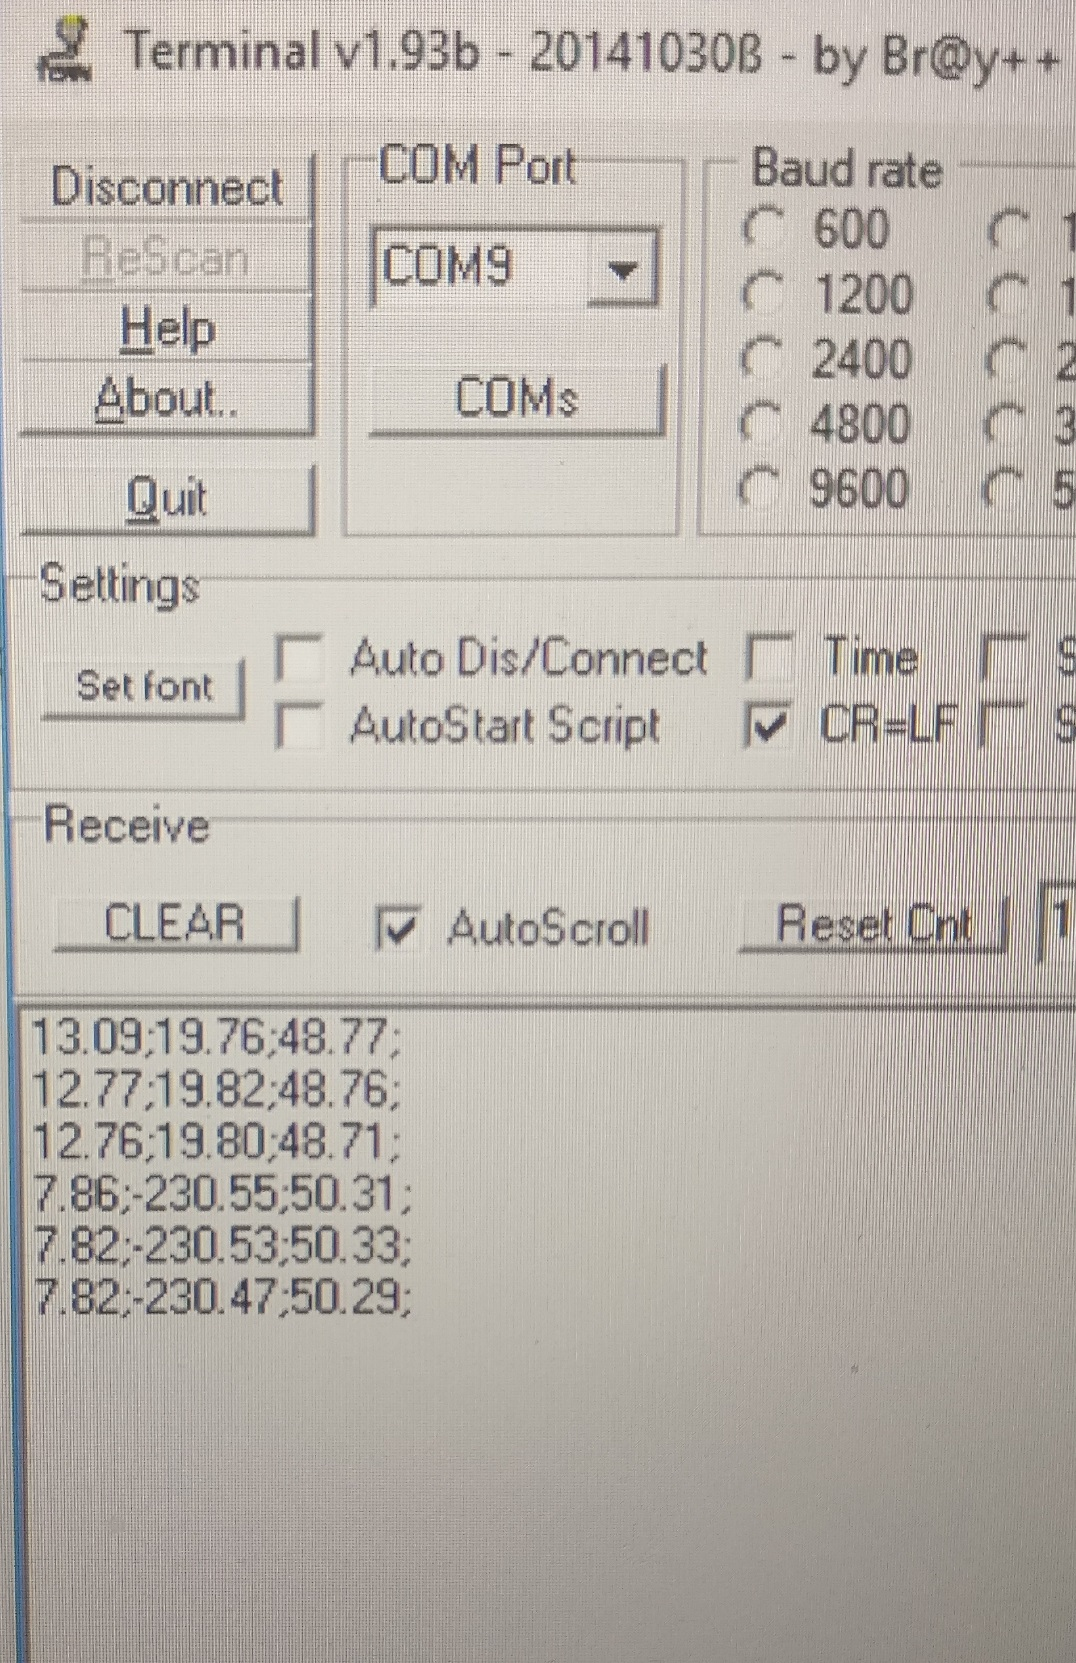
\includegraphics[width=0.245\textwidth]{./img/bob/midCoilField.jpg}
     }
    % \hfill
     \caption*{Fonte: Autor.}\label{fig:CurFieldMd}
\end{figure}


\begin{figure}[H]
    \centering
     \caption{Medidas de resistência e indutância na bobina externa}
     \subfloat[Valor da resistência medida ($\Omega$)]{%
        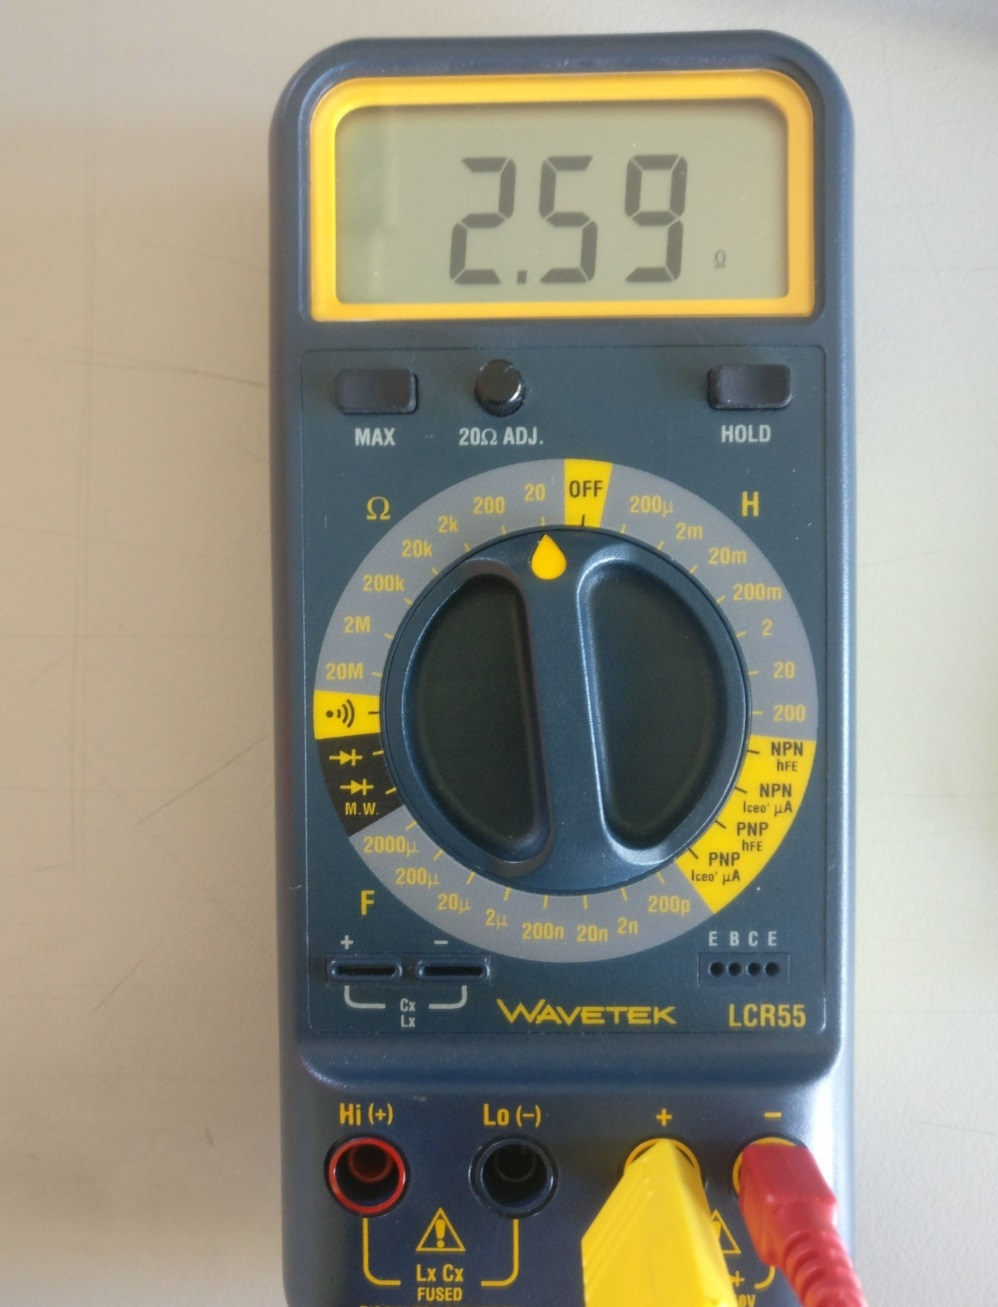
\includegraphics[width=0.25\textwidth]{./img/bob/externalCoilResistance.jpg}
     }
     \subfloat[Valor da indutância medida (mH)]{%
        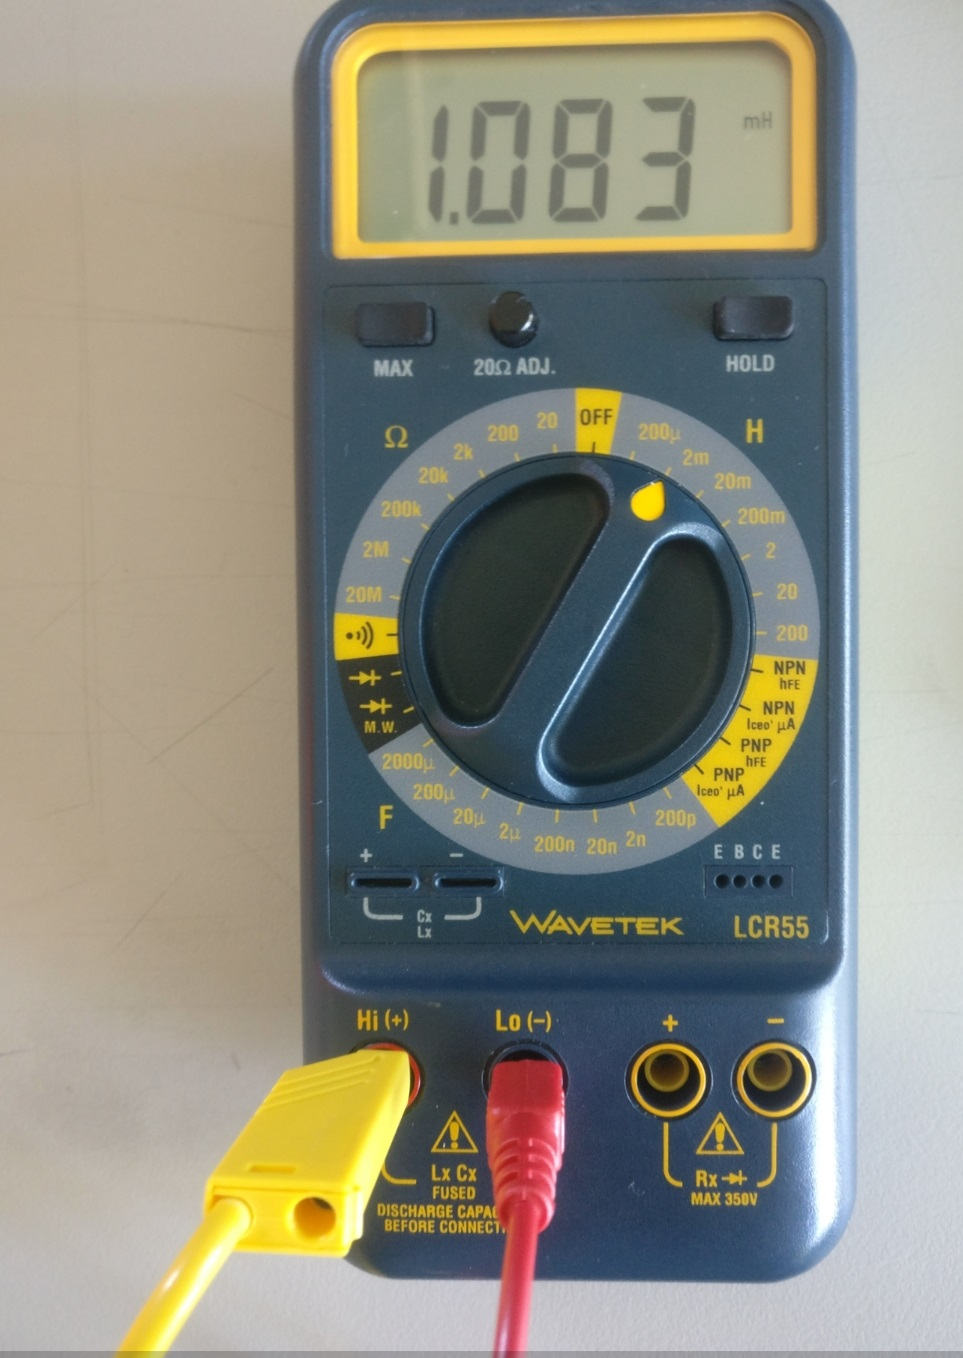
\includegraphics[width=0.235\textwidth]{./img/bob/externalCoilInductance.jpg}
     }
    % \hfill
     \caption*{Fonte: Autor.}\label{fig:ResIndEx}
\end{figure}

\begin{figure}[H]
    \centering
     \caption{Estimação do campo gerado pela bobina interna}
     \subfloat[Tensão e corrente da fonte]{%
        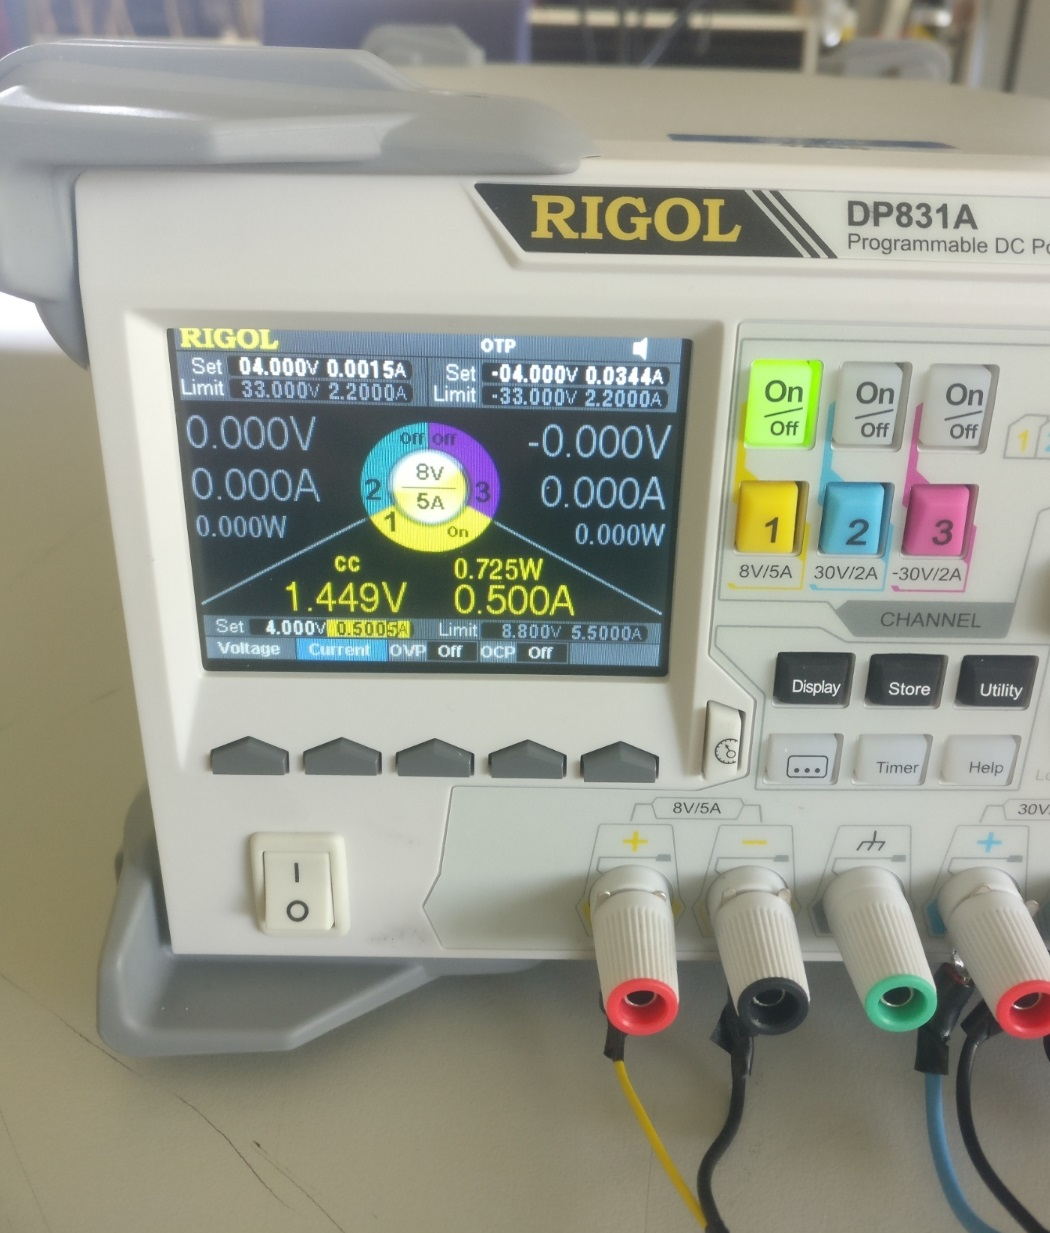
\includegraphics[width=0.35\textwidth]{./img/bob/externalCoilCurrent.jpg}
     }
     \subfloat[Valores de campo recebidos no computador]{%
        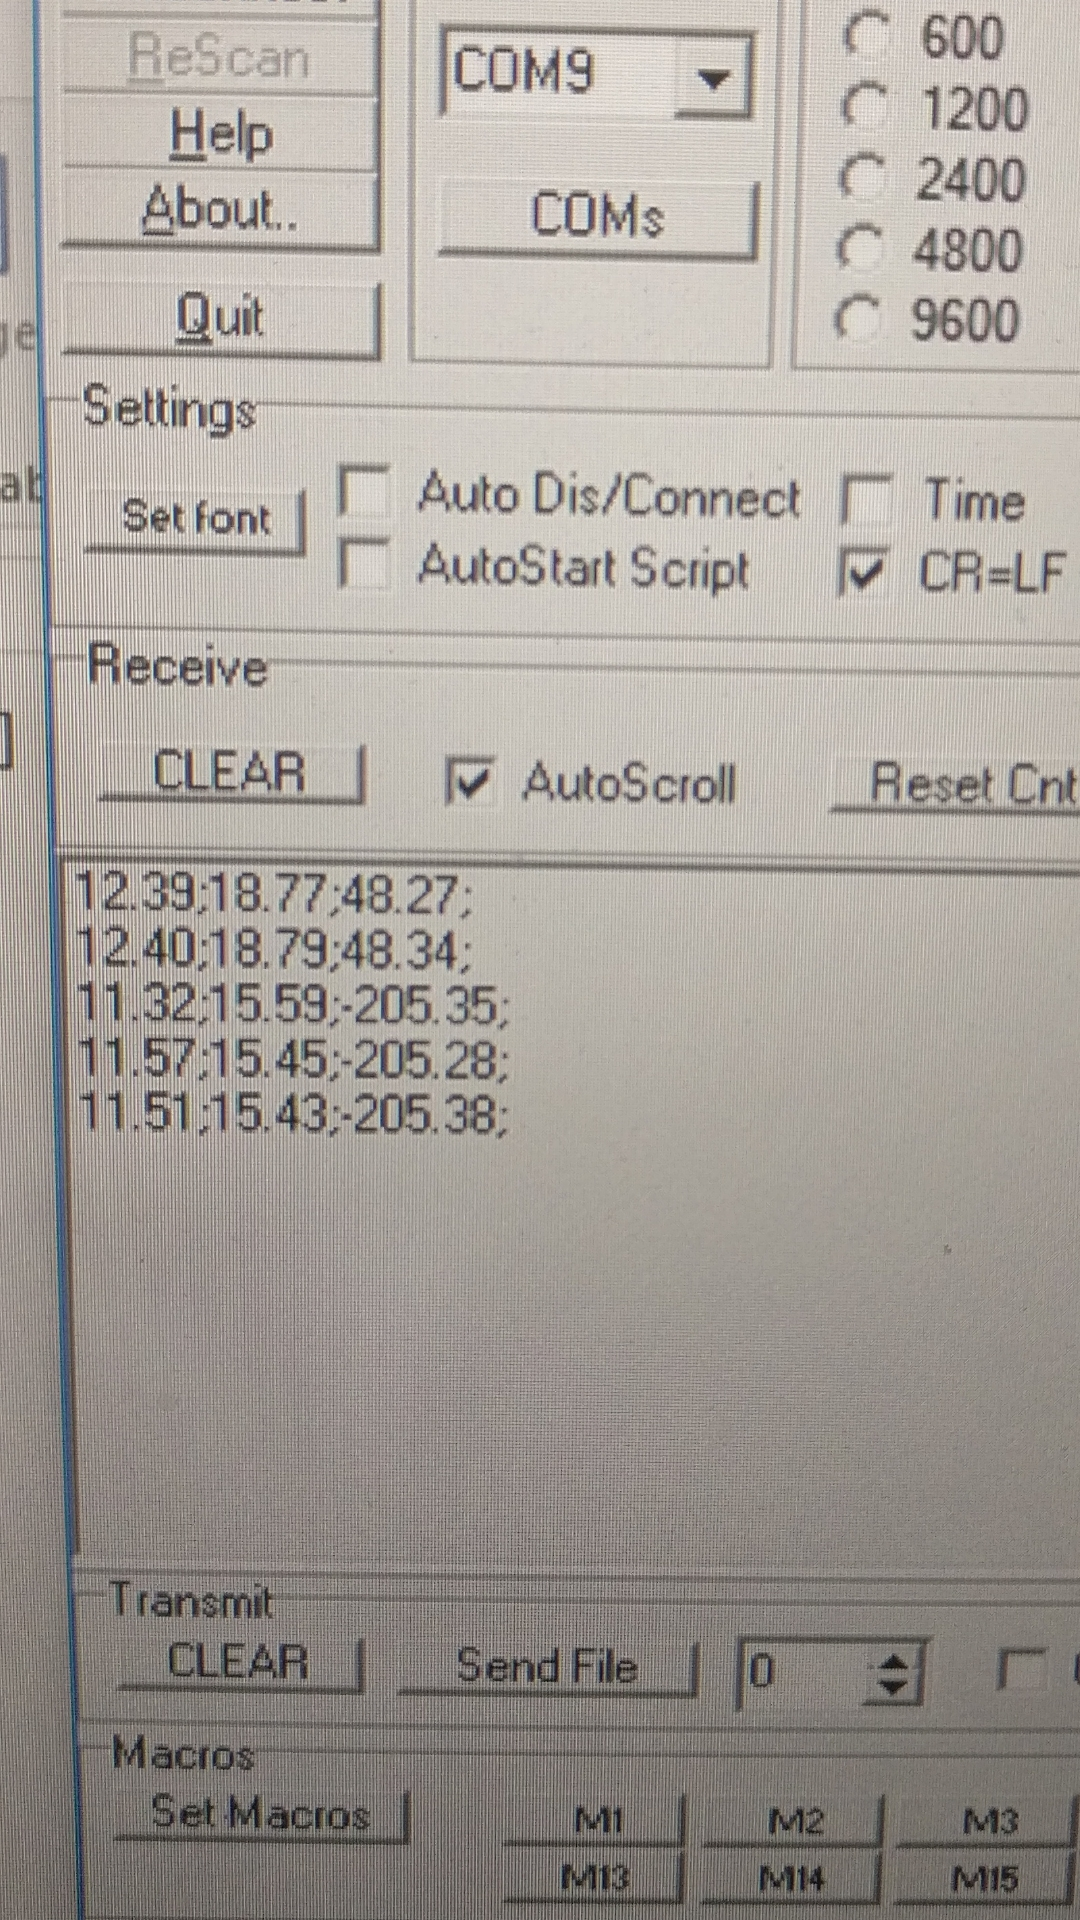
\includegraphics[width=0.23\textwidth]{./img/bob/externalCoilField.jpg}
     }
    % \hfill
     \caption*{Fonte: Autor.}\label{fig:CurFieldEx}
\end{figure}
Fazendo uma breve comparação entre os valores teóricos e estimados com os valores medidos, chegaram-se aos erros encontrados na figura \ref{fig:err}, essas informações são melhores apresentadas nas tabelas \ref{tab:intCoil}, \ref{tab:midCoil} e \ref{tab:extCoil}.
Com base nessas informações é possível considerar que os métodos utilizados permitiram gerar um campo em cada bobina na direção desejada, alinhados com o sensor. Há um erro de amplitude menor que 2\% em todas as bobinas, o que é aceitável para este projeto. Os valores de resistência ficaram bem diferentes do estimado. Porém, a influência desse parâmetro não afeta de forma significativa o equipamento e pode ser desprezada.

A indutância foi medida para possíveis alterações no funcionamento das bobinas, não sendo relevante para este trabalho. 

\begin{figure}[H]
    \centering
     \caption{Erros encontrados no módulo de campo da bobina }
     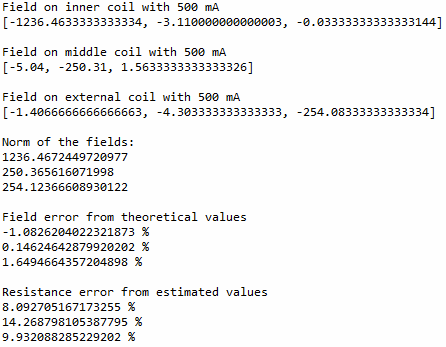
\includegraphics[width=0.8\textwidth]{./img/bob/fieldErr.png}
     \caption*{Fonte: Autor.}\label{fig:err}
\end{figure}

\begin{table}[H]
    \centering
    \caption{Informações da bobina (Interna)}
    \begin{tabular}{|c|c|c|c|}
     \hline
     \textbf{Parâmetro} & \textbf{Valores estimados} & \textbf{Valores medidos} & \textbf{erro}\\
     \hline
     Resistência&  5.26 $\Omega$  & 5.69 $\Omega$ & 8.09 \% \\ 
     Campo induzido &   1250.00 $\mu$T  & 1236.47 $\mu$T & -1.08 \% \\ \hline
     
    \end{tabular}
    \label{tab:intCoil}
\end{table}

\begin{table}[H]
    \centering
    \caption{Informações da bobina (Intermediária)}
    \begin{tabular}{|c|c|c|c|}
     \hline
     \textbf{Parâmetro} & \textbf{Valores estimados} & \textbf{Valores medidos} & \textbf{erro}\\
     \hline
     Resistência&  1.69 $\Omega$  & 1.93 $\Omega$ & 14.27 \% \\ 
     Campo induzido &  250.00 $\mu$T  & 250.36 $\mu$T & 0.15 \% \\ \hline
     
    \end{tabular}
    \label{tab:midCoil}
\end{table}

\begin{table}[H]
    \centering
    \caption{Informações da bobina (Exterior)}
    \begin{tabular}{|c|c|c|c|}
     \hline
     \textbf{Parâmetro} & \textbf{Valores estimados} & \textbf{Valores medidos} & \textbf{erro}\\
     \hline
     Resistência&  2.36 $\Omega$  & 2.59 $\Omega$ & 9.93 \% \\ 
     Campo induzido &   250.00 $\mu$T  & 254.12 $\mu$T & 1.65 \% \\ \hline
     
    \end{tabular}
    \label{tab:extCoil}
\end{table}

Dois testes foram feitos para determinar o comportamento do campo gerado através da observação de uma bussola. No primeiro teste foi feito um \textit{script} em \textit{python} que compensava o campo magnético terrestre e em seguida gerava um campo circular no plano xy. O efeito desse sinal magnético sendo aplicado na bussola fazia com que a mesma ficasse com seu ponteiro girando de forma circular e com velocidade angular constante, na faixa de alguns Hertz.

Observando-se esse primeiro teste era possível determinar se o sistema estava controlando as bobinas da maneira correta, não vendo nenhum tipo de mudança abrupta na movimentação da bússola por exemplo.

Outro teste realizado foi a compensação total do campo magnético da terra. A bussola era sensível o suficiente para detectar campos de cerca de 2 $\mu T$. Foi feito um \textit{script} em \textit{python} que apenas compensava o campo magnético terrestre. Após compensado a bussola era colocada no centro da região de campo uniforme. Com a bússola no centro da estrutura um imã era aproximado fazendo com que a mesma apontasse para o imã. Como não havia nenhum campo resultante, assim que o imã era afastado da bussola, a mesma permanecia apontada para a direção que o imã estava. Após esse teste a corrente das bobinas eram desligadas e a bússola voltava a apontar para o norte terrestre, mostrando que o sistema era capaz de anula o campo magnético terrestre. Na figura \ref{fig:compass} pode-se observar uma ilustração da bússola no centro da estrutura.


\begin{figure}[H]
    \centering
     \caption{Ilustração da bússola no centro da estrutura das bobinas}
     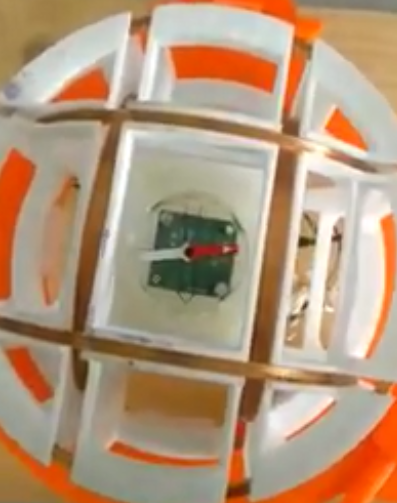
\includegraphics[width=0.4\textwidth]{./img/compass.png}
     \caption*{Fonte: Autor.}\label{fig:compass}
\end{figure}